\section{Complete Cooperative Policy-Learning Transfer Results}
Held-out MAPPO transfer studies match message/environment budgets and charge a disjoint critic-residual probe that selects participation without evaluation return.
Both studies use eight fresh seeds per dependence regime and compare against fixed $q\in\{1,2,4,8\}$.
We compare regime-wise fixed envelopes and the strongest single fixed action for an unknown regime.

In PettingZoo \texttt{simple\_spread\_v2}, the controller commits to $q=8$ in all eight independent-stream runs and $q=1$ in all eight shared-stream runs.
It lies within $0.357$ and $0.889$ percent of the corresponding regime-wise fixed envelopes.
Against the strongest single fixed action, $q=8$, the mean of the regime--seed normalized AUC gains is $2.319$ percent; normalization precedes averaging.

In MaMuJoCo \texttt{HalfCheetah-v2/2x3}, the task-specific prespecified catalogue is $\{2,8\}$, while evaluation still includes all four fixed actions.
The controller selects $q=8$ in all eight independent-stream runs and $q=2$ in all eight shared-stream runs.
Relative to the corresponding regime-wise fixed envelopes, its AUC changes are $-0.542$ and $-0.997$ percent, both within the prespecified two-percent noninferiority margin.
When the regime is unknown, the strongest single fixed action is $q=8$.
Forming each seed's equal-regime mixture before normalization gives a mean paired AUC gain of $8.341$ percent, a one-sided 95 percent lower bound of $1.107$ percent, seven of eight positive pairs ($p=0.0352$), and a final-return gain of $4.637$ percent.

Fig.~\ref{fig:marl-return} shows the unsmoothed deterministic team-return curves against the maximum charged dual-budget fraction.
Probes consume at most $0.768$ percent of messages; selection overhead is below $10^{-6}$ of training time.
\begin{figure*}[t]
\centering
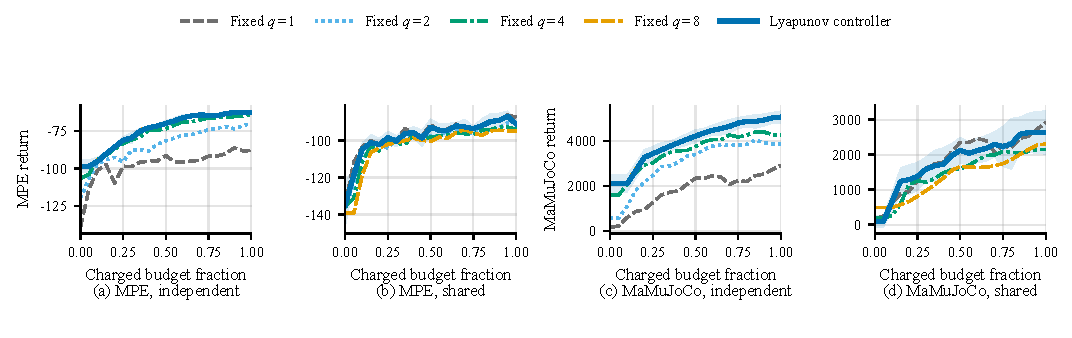
\includegraphics[width=0.96\textwidth]{figures/marl_multienvironment_returns.pdf}
\caption{Fully charged MAPPO team-return learning curves on two cooperative environments with fixed $q\in\{1,2,4,8\}$ and the Lyapunov probe-then-commit controller (eight held-out seeds per regime; shaded bands are controller 95 percent confidence intervals).
The controller selects $q=8$ for independent streams in both environments, $q=1$ for shared MPE streams, and $q=2$ for shared MaMuJoCo streams.}
\label{fig:marl-return}
\end{figure*}
